\documentclass[a4paper, 12pt, report]{lifestyle}

\usepackage{rcs}
\usepackage[top=3.6cm,bottom=3.6cm,right=3.2cm,left=3.5cm]{geometry}
\usepackage{bm}

\RCS $Revision: 1.8 $
\RCS $Date: 2012-08-16 17:00:00$
\RCS $State: Exp $

%%%%%%%%%%%%%%%%%%%%%%%%%%%%%%%%%%%%%%%%%%%%%%%%%%%%%%
% New user defined commands
%%%%%%N%%%%%%%%%%%%%%%%%%%%%%%%%%%%%%%%%%%%%%%%%%%%%%%%

%\newcommand{\Div} {\operatorname{div}}
\newcommand{\Grad} {\boldsymbol{\nabla}}
\newcommand{\strain}{{\uu \epsilon}}
\newcommand{\Strain}[1] {(\Grad{\uu{#1}} +  (\Grad{\uu{#1}})^T )/2 }
\newcommand{\piola}{\uu \sigma_\ms}

\newcommand{\St}{\operatorname{Stokes}}
\newcommand{\NS}{\operatorname{Fluid}}
\newcommand{\Str}{\operatorname{Str}}

\newcommand{\uu}[1]{\boldsymbol{#1}}
\newcommand{\U}{{\uu{u}}}
\newcommand{\V}{{\uu{v}}}
\newcommand{\bY}{{\hat {\uu x}}}
\newcommand{\bw}{{\uu w}}
\newcommand{\D}{{\uu d}}
\newcommand{\Df}{{\uu d^\mf}}
\newcommand{\Ds}{{\uu d^\ms}}
\newcommand{\R}{\mathbb{R}}
\newcommand{\N}{\mathbb{N}}


\newcommand{\Div}{\operatorname{div}}
\newcommand{\dis}{\displaystyle}

%

\newcommand{\xs}{\uu x^\ms}
\newcommand{\xf}{\uu x^\mf}
\newcommand{\ds}{\uu d^\ms}
\newcommand{\df}{\uu d^\mf}
\newcommand{\mf}{{\mathrm{f}}}
\newcommand{\ms}{{\mathrm{s}}}
\newcommand{\wf}{\uu w^\mf}
\newcommand{\ws}{\uu w^\ms}
\newcommand{\disp}[1]{\lambda^{#1}}
%\newcommand{\Omegat}[1][t]{\Omega(#1)}
%
% FSI commands
%
\newcommand{\hOmega} {\hat\Omega}
\newcommand{\hOmegaF}{\hat{\Omega}^{\mf}}
\newcommand{\hOmegaS}{\hat\Omega^{\ms}}
\newcommand{\hGamIn} {\hat\Gamma^{\mathrm{in}}}
\newcommand{\hGamOu} {\hat\Gamma^{\mathrm{out}}}
%
\newcommand{\Omegat}{\Omega(t)}
\newcommand{\Omegai}{\Omega_0}
\newcommand{\OmegaF} {\Omega^{\mf}}
\newcommand{\OmegaFi} {\Omega_0^{\mf}}
\newcommand{\OmegaFt}{\Omega^{\mf}(t)}
\newcommand{\OmegaS} {\Omega^{\ms}}
\newcommand{\OmegaSi} {\Omega_0^{\ms}}
\newcommand{\OmegaSt}{\Omega^{\ms}(t)}
%
\newcommand{\Domt}   {\Omega(t)}
\newcommand{\Domi}   {\Omega_0}
\newcommand{\DomF}   {\Omega^{\mf}}
\newcommand{\DomFi}  {\Omega_0^{\mf}}
\newcommand{\DomFt}  {\Omega^{\mf}(t)}
\newcommand{\DomS}   {\Omega^{\ms}}
\newcommand{\DomSi}  {\Omega_0^{\ms}}
\newcommand{\DomSt}  {\Omega^{\ms}(t)}
\newcommand{\GamIn}  {\Gamma^{\mathrm{in}}}
\newcommand{\GamIni}  {\Gamma^{\mathrm{in}}_0}
\newcommand{\GamInt} {\Gamma^{\mathrm{in}}(t)}
\newcommand{\GamOu}  {\Gamma^{\mathrm{out}}}
\newcommand{\GamOui}  {\Gamma^{\mathrm{out}}_0}
\newcommand{\GamOut} {\Gamma^{\mathrm{out}}(t)}
\newcommand{\GamFS}[1] {\Gamma(t^{#1})}
\newcommand{\GamFSi} {\Gamma_0}
\newcommand{\GamFSt} {\Gamma(t)}
\newcommand{\hGamW}  {\Sigma_0}
\newcommand{\Wall}   {\Sigma}
\newcommand{\Wallt}  {\Sigma(t)}
\newcommand{\hWall}  {\Sigma^s}
%\newcommand{\ALE}[1]{{\CMcal A}_{#1}}
\newcommand{\ALE}[1]{{\uu x^\mf_{#1}}}
\newcommand{\diffALE}[1]{\left.\frac{\partial #1}{\partial t}\right|_{\uu x_0}}
\newcommand{\In}{{\operatorname{in}}}
\newcommand{\Out}{{\operatorname{out}}}
\newcommand{\Fstress}[1][{ }] {\uu{\sigma}_\mf (\U^{#1}, p^{#1})}
\newcommand{\Sstress}[1][{ }] {\uu{\sigma}_\ms}
%
% FSI operators
%
\newcommand{\Sf}{S_\mf}
\newcommand{\Ss}{S_\ms}
\newcommand{\SFprime}{S'_\mf}
\newcommand{\SSprime}{S'_\ms}
\newcommand{\DN}{S'_\ms(\lambda^k)}
\newcommand{\ND}{S'_\mf(\lambda^k)}
\newcommand{\NN}{S'_\mf(\lambda^k) + S'_\ms^{-1}(\lambda^k)}
\newcommand{\invDN}{{S'}_\ms^{-1}(\lambda^k)}
\newcommand{\invND}{{S'}_\mf^{-1}(\lambda^k)}
\newcommand{\invNN}{{S'}_\mf^{-1}(\lambda^k) + S'_\ms^{-1}(\lambda^k)}



\title{\lifetitle{LifeV User Manual}
{G. Fourestey, S. Deparis}
}
\date{}
\makeindex
\makeglossary

\pagestyle{fancy}

%%\includeonly{lifev-dev_generalities,lifev-dev_howto}
\begin{document}

\maketitle

\phantom{dummy text}
\vfill
This manual is for LifeV (version 2.2.1, March 2012), %1.3.1, October 2010), 
a library for scientific computing 
using finite elements, specially aimed at fluid-structure interaction and blood flow simulation.

Copyright (C) 2001- 2012 EPFL, INRIA, Polytechnico Di Milano.

\tableofcontents

%\listoffigures

\listoftables


\chapter{Generalities}
\label{cha:generalities}

\section{Scope of the document}
\label{sec:scope-document}

This is an informal document dedicated to amateur or inexperienced users of the
software library \thelibrary (life 5).

The major objectives of this document are:
\begin{enumerate}
\item to compile the software library,
\item to provide examples of its use.
\end{enumerate}
For a more detailed overview of \lifev's main features (management of boundary conditions, time and space discretization, algebraic solvers and preconditioners, etc), see the doxygen webpage: \url{https://cmcsforge.epfl.ch/doxygen/lifev/}.
\section{Language and nomenclature convention}
\label{sec:lang-nomencl-conv}

\texttt{typesetting font style} is used to indicate parts of
computer code, configure shell scripts, command-prompt instructions and webpages.

\section{Software Management}
\label{sec:software-management}

The software source, its documentation and all related documents (this
one included) are kept in a repository under revision control
using \verb!git!\ixns{git}{versioning}\footnote{git is the fast version control system.}. Its goal
is to provide tools to manage software development in a concurrent environment.
See \url{http://git-scm.com/documentation}
for a tutorial.

As mentioned above, a website {\it\`a la} Sourceforge\footnote{\url{http://www.sourceforge.net}}
\url{http://cmcsforge.epfl.ch} has been set up
to host the source code and help the software management.
It requires that you open an account\footnote{\url{https://cmcsforge.epfl.ch/account/register.php}}
there and ask to join the project \lifev using the link at the
bottom of the developers' list.
Once you would become a member, you will gain access to all the facilities:
tracker, task manager, git repository, forums, document manager and a few other
tools which are very useful if not absolutely essential to such a project.

Finally, if you expect a frequent use of the \verb!git!\ixns{git}{versioning} repository
we recommend to costumize the
\verb!ssh! and \verb!ssh-agent!
 in order to gain acces  without the need to type your password everytime you issue
a command. Please refer to \url{http://mah.everybody.org/docs/ssh} in order to configure
your ssh agent.

We advice every user to apply to the list lifev-users on \url{http://groups.google.com}
where one can get in touch with other users and developers.

\section{Compiling LifeV}
\label{compile-lifev}

There are a few compilation tools and libraries we need to build and install before
compiling \lifev, here is a short presentation. Note that, in addition to the following description, the complete installation steps are available on the following webpages:
\begin{enumerate}
\item \url{http://www.lifev.org/documentation/installation-tutorial}\,,
\item \url{https://cmcsforge.epfl.ch/projects/lifev/wiki/LifeV_on_MacOSX}\,.
\end{enumerate}



In computer science, a library is a set of subroutines or classes used to develop software.
Usually they are downloaded as a so called ``tarball" file
compressed using the \verb!tar! command. There are different ways to compress
libraries but the most common is to use the command \verb!tar -cvf! and further compress
``zip" it with \verb!gzip!. If your tarball has the suffix \verb!.tar.gz! equivalent to \verb!.tgz!,
you can decompress ``unzip" it with \verb!gunzip! followed by the name of the \verb!.tar.gz! file and
extract its contents using \verb!tar -xvf! followed by the name of the \verb!.tar! file.
If you find the libraries compressed with other formats
please refer to the unix manuals \verb!man! or the numerous
on-line documents for further information.

Software libraries need to be extracted, compiled and installed. In unix-like
systems, the libraries \verb!.a! and
\verb!.so! files are installed usually in the directory \verb!/usr/lib!,
 while header files
\verb!.h! are installed in the \verb!/usr/include! directory. Compilers search
for libraries there by default, but in principle they can be installed anywhere you want
as long as you pass the path to the library using the compiler flag \verb!-L! immediately
followed by the library path (e.g. \verb!-L/path/to/lib!) and similarly for the header files using the compiler
flag \verb!-I! followed by the include path. Libraries compiled from source are usually installed in \verb!/usr/local/lib!, \verb!/usr/local/include!.

Libraries are usually created with the prefix \verb!lib! followed by the name of the library
and linked with the compiler flag \verb!-l! followed by its name (e.g. \verb!-lblas!).

\subsubsection{Compilation Environment}
\label{sec:comp-envir}

\lifev depends on a number of tools at compilation time that are part
of the \ix{autotools} from the GNU project\footnote{\url{http://www.gnu.org}}
available in most Linux OS:

\begin{itemize}
\item \verb!g++-4.0!\ixns{g++}{compilers} or newer (currently \verb!4.9.2!).
\item \verb!mpi!\ixns{mpi}{compilers}, with preference to \verb!openmpi!\ixns{openmpi}{compilers}.
\item \verb!CMake 2.8.11! or newer (currently \verb!3.1.0!).
\end{itemize}

In Mac OS X you get gcc in Xcode and cmake can be installed using MacPorts with the command \verb!sudo port install cmake!. You can check the version of a command typing the command followed by \verb!--help!,
for example type \verb!cmake --help!.

\lifev depends on several optimized libraries, you can check if you have them installed
using the \verb!locate! command (after updating the search database with \verb!sudo updatedb!) followed by the name of the library, for example
\verb!locate liblapack.a!, or go to the \verb!/usr/lib! directory and search on the
list with \verb!ls!.
It is important to notice that some libraries are linked to others and they should
be compatible, therefore you should build them in the order of dependency and with
compatible flags and compilers.

These are the optimized libraries you need to have installed:

\begin{itemize}
\item A version of \verb!MPI!.
The message passing interface for C and Fortran compilers. For example \url{http://www.open-mpi.org/}.
Once installed you can check the necessary flags for its use by typing
\verb!mpicc --show!.\\
On a Debian system the command \verb!sudo apt-get install libopenmpi*! should do the trick.\\
In Mac OS X using MacPorts install a fortran compiler typing
\verb!sudo port install gcc46! and openmpi with \verb!sudo port install openmpi!. Note however that MPI should be natively installed if you installed XCode.

\item \verb!BOOST!.
Libraries which extend the functionality of C$++$. Check if they exist on your computer, they are many
libraries with the prefix \verb!libboost!.\\
If you need to install them, try \verb!sudo apt-get install libboost*! on Debian systems or
something similar for other Linux distros.\\
In Mac OS X using MacPorts type \verb!sudo port install boost!.\\
If you need to compile from source, download the libraries at \url{http://www.boost.org}.
Make sure you include the line ``\verb!using mpi;!" in the configuration text file \verb!project-config.jam!.
You can specify the path to install using the flag \verb!--prefix=/path/! when running \verb!./bjam!
\verb!install!. But most of the time cross compilation of this library won't work completely.

\item \verb!HDF5!
If you don't have the library hdf5 installed in your system, you could use the
\verb!sudo! \verb!apt-get install libhdf5-openmpi-dev! command on Debian systems or something similar
for your particular distro. There are detailed instructions on-line on how to build it for other systems and
with other options, see \url{http://micro.stanford.edu/wiki/Install_HDF5#Build_and_Installation_from_Sources}.\\
In Mac OS X using MacPorts type \verb!sudo port install hdf5! or build it from the sources to link it to the correct
openmpi compilers.

\item \verb!BLAS!.
On Debian systems run \verb!sudo apt-get install libblas-dev!.\\
In Mac OS X
the system comes with blas and lapack as part of the Accelerate framework \verb!-framework Accelerate!,
and if using MacPorts type
\verb!sudo port install atlas! to install the atlas library (blas and lapack).\\
To compile from source, get the libraries e.g.\ at \url{https://www.tacc.utexas.edu/research-development/tacc-software/gotoblas2}. To build just type \verb!make!.
To make use of the library remember to
have the pthreads library and flag  \verb!-lpthread! while linking to the blas library  \verb!libgoto2_xxxxx_xx.xx.a!,
whose exact name depends on the characteristics of your hardware.

\item \verb!LAPACK!.
Fortran $90$ Linear Algebra Routines for systems of simultaneous linear algebra equations, linear least-squares problems
and matrix eigenvalue problems. You must pay attention to build the lapack using an optimized blas like the GotoBLAS (see above). Download it at \url{http://www.netlib.org/lapack/}. You need a fortran compiler (for example \verb!gfortran!).
Copy \verb!make.inc.example! to \verb!make.inc! and edit the path to the blas library followed by the flag \verb!-lpthread!
and type \verb!make!.\\
For a non-optimized version on a Debian system run \verb!sudo apt-get install liblapack-dev!.

\item \verb!PARMETIS!.
You can download ParMetis from \url{http://glaros.dtc.umn.edu/gkhome/metis/parmetis/download}. Set \verb!CC=mpicc!
in \verb!Makefile.in!. and type \verb!make!. In Mac OS X you need the include path flags
\verb!-I/usr/include! and \verb!-I/usr/include/malloc!.

\item \verb!UMFPACK (now part of SuiteSparse)!.
Set of routines for solving unsymmetric sparse linear systems.\\
On a Debian system, install it with the command \verb!sudo apt-get install libsuitesparse-dev!.
To compile SuiteSparse from source, download it from \url{http://faculty.cse.tamu.edu/davis/suitesparse.html} and follow the instructions in the \verb!README.txt! file (in particular, you'll want to edit the \verb!SuiteSparse_config/SuiteSparse_config.mk! file according to your configuration).\\
For Mac OS X you must uncomment the special options given for this system, so you can use the blas and lapack
from atlas or from the Accelerate framework \verb!-framework Accelerate!.

\item \verb!TRILINOS!\ixns{aztec}{algebra}. See the next section.

\end{itemize}

\subsection{Trilinos compilation}
\lifev depends on Trilinos, a set of object oriented C$++$ interfaces for packages like
blas, lapack, parmetis, umfpack and many more. A copy of the source
code is available for download at \url{http://trilinos.org/download/}.

After downloading, decompressing and extracting the tarball, you'll need to
make a build directory anywhere you want to avoid build in the sources directory. (in the
following script, we assume that the directories \verb!trilinos! and \verb!trilinos-build! are at the same level)
Trilinos (latest version $11.12.1$ at the time of writing) now requires the CMake
build system $2.8.11$ or newer.
Go to the build directory and write a \verb!do-configure! shell script like the following


\begin{lstlisting}
#!/bin/bash

EXTRA_ARGS=$@

cmake \
    -D CMAKE_BUILD_TYPE:STRING=RELEASE \
    -D Trilinos_ENABLE_Amesos:BOOL=ON \
    -D Trilinos_ENABLE_Anasazi:BOOL=ON \
    -D Trilinos_ENABLE_AztecOO:BOOL=ON \
    -D Trilinos_ENABLE_Belos:BOOL=ON \
    -D Trilinos_ENABLE_Epetra:BOOL=ON \
    -D Trilinos_ENABLE_EpetraExt:BOOL=ON \
    -D Trilinos_ENABLE_Galeri:BOOL=OFF \
    -D Trilinos_ENABLE_Ifpack:BOOL=ON \
    -D Trilinos_ENABLE_Isorropia:BOOL=OFF \
    -D Trilinos_ENABLE_Kokkos:BOOL=ON \
    -D Trilinos_ENABLE_ML:BOOL=ON \
    -D Trilinos_ENABLE_TESTS:BOOL=OFF \
    -D Trilinos_ENABLE_Teuchos:BOOL=ON \
    -D Trilinos_ENABLE_ThreadPool:BOOL=ON \
    -D Trilinos_ENABLE_Tpetra:BOOL=ON \
    -D Trilinos_ENABLE_Triutils:BOOL=ON \
    -D Trilinos_ENABLE_Zoltan:BOOL=ON \
    \
    -D Trilinos_EXTRA_LINK_FLAGS:STRING="-lpthread" \
    -D TPL_ENABLE_Pthread:BOOL=ON \
    \
    -D TPL_ENABLE_BLAS:BOOL=ON \
    -D BLAS_INCLUDE_DIRS:PATH=/blas/include/dir/ \
    -D BLAS_LIBRARY_DIRS:PATH=/blas/lib/dir/ \
    -D BLAS_LIBRARY_NAMES:STRING="blas" \
    \
    -D TPL_ENABLE_LAPACK:BOOL=ON \
    -D LAPACK_INCLUDE_DIRS:PATH=/lapack/include/dir/ \
    -D LAPACK_LIBRARY_DIRS:PATH=/lapack/lib/dir/ \
    -D LAPACK_LIBRARY_NAMES:STRING="lapack" \
    \
    -D TPL_ENABLE_HDF5:BOOL=ON \
    -D HDF5_INCLUDE_DIRS:PATH/hdf5/include/dir/ \
    -D HDF5_LIBRARY_DIRS:PATH=/hdf5/lib/dir/ \
    \
    -D TPL_ENABLE_UMFPACK:BOOL=ON \
    -D UMFPACK_INCLUDE_DIRS:PATH=/umfpack/include/dir/ \
    -D UMFPACK_LIBRARY_DIRS:PATH=/umfpack/lib/dir/ \
    -D UMFPACK_LIBRARY_NAMES:STRING="umfpack;amd" \
    \
    -D TPL_ENABLE_MPI:BOOL=ON \
    -D MPI_BASE_DIR:PATH=/usr/lib/openmpi/ \
    -D MPI_BIN_DIR:PATH=/usr/bin \
    \
    -D TPL_ENABLE_ParMETIS:BOOL=ON \
    -D ParMETIS_LIBRARY_DIRS:PATH=/parmetis/lib/dir/ \
    \
    -D CMAKE_INSTALL_PREFIX:PATH=./ \
    $EXTRA_ARGS \
    ../trilinos/
\end{lstlisting}

Simply modify the paths of libraries according to your particular configuration and run the shell script (\verb!chmod +x do-configure && ./do-configure!). For example, instead of \verb!lapack_library_name! you should type the name of your lapack library without the
\verb!lib! prefix and the \verb!.a! suffix. The prefix and suffix are automatically added by CMake.\\
If SuiteSparse was compiled from source the \verb!UMFPACK_LIBRARY_NAMES! variable has to be modified so that it reads \verb!"umfpack;suitesparseconfig;cholmod;colamd;amd"!\\
As an alternative to the above script, you can run
\begin{lstlisting}
ccmake ../lifev
\end{lstlisting}
to get a graphical configuration menu (however \verb!ccmake! needs \verb!libncurses! to be installed), with many more options.

After the configuration is done, just type
\begin{lstlisting}
make
\end{lstlisting}
that  will compile the static files and further
\begin{lstlisting}
make install
\end{lstlisting}
that will create and install the library files
in two subdirectories \verb|lib| and \verb|include|, where
it will respectively pack the objects files into library files (.a and .la files)
and copy the include files ( .h or .hpp files ).

The Trilinos library is now installed in the build directory you created.

\subsection{Compilation from git}
\label{sec:compile-cvs}
You need first to have an account on \url{http://cmcsforge.epfl.ch} and
be part of the \lifev project, see~\ref{sec:software-management}.

First, you need to checkout \lifev. \verb!git! has
been configured to use \ixv{ssh} and your \verb!ssh! keys to
access the repository via \verb!ssh! without entering your password. When your ssh agent is properly configured,
send your public key to the local administrator, such that it can be included in
the gitolite configuration.
Then you will be able to access the
repositories without password.

It is now time to download and compile the code.
Just type
\begin{lstlisting}
git clone git@cmcsforge.epfl.ch:lifev.git lifev
\end{lstlisting}
and go to the newly created directory
\begin{lstlisting}
cd lifev
\end{lstlisting}

Second, you must make a build directory apart from the
lifev sources directory, for example in your home you can have a
\verb!lib! directory with a \verb!lifev! subdirectory and further
an optimized version subdirectory \verb!opt! or the debugging mode
subdirectory \verb!debug!, or something similar according to your own taste.

Third, you have to execute the following
\verb+do-configure+ shell script (again, modified to suite your configuration) in the \verb!opt! directory.
It will automatically check the availability of the needed components
for \lifev compilation :


\begin{lstlisting}
#!/bin/bash

EXTRA_ARGS=$@

TRILINOS_BUILD_DIR=/trilinos/build/dir/

cmake \
-D CMAKE_BUILD_TYPE:STRING=RELEASE \
\
-D TPL_ENABLE_MPI:BOOL=ON \
\
-D ParMETIS_INCLUDE_DIRS:PATH=/parmetis/include/dir/ \
-D ParMETIS_LIBRARY_DIRS:PATH=/parmetis/lib/dir/ \
\
-D TPL_ENABLE_BLAS:BOOL=ON \
-D BLAS_INCLUDE_DIRS:PATH=/blas/include/dir/ \
-D BLAS_LIBRARY_DIRS:PATH=/blas/lib/dir/ \
-D BLAS_LIBRARY_NAMES:STRING="blas" \
\
-D TPL_ENABLE_LAPACK:BOOL=ON \
-D LAPACK_INCLUDE_DIRS:PATH=/lapack/include/dir/ \
-D LAPACK_LIBRARY_DIRS:PATH=/lapack/lib/dir/ \
-D LAPACK_LIBRARY_NAMES:STRING="lapack" \
\
-D TPL_ENABLE_HDF5:BOOL=ON \
-D HDF5_INCLUDE_DIRS:PATH=/hdf5/include/dir/ \
-D HDF5_LIBRARY_DIRS:PATH=/hdf5/lib/dir/ \
\
-D TPL_ENABLE_Boost:BOOL=ON \
-D Boost_INCLUDE_DIRS:PATH=/boost/include/dir/ \
\
-D TPL_ENABLE_Trilinos:STRING=ON \
-D Trilinos_DIR:PATH=$TRILINOS_BUILD_DIR/lib/cmake/Trilinos \
-D Trilinos_INCLUDE_DIRS:PATH=$TRILINOS_BUILD_DIR/include/ \
-D Trilinos_LIBRARY_DIRS:PATH=$TRILINOS_BUILD_DIR/lib/ \
\
-D LifeV_VERBOSE_CONFIGURE:BOOL=OFF \
-D CMAKE_VERBOSE_MAKEFILE:BOOL=OFF \
\
-D LifeV_ENABLE_STRONG_CXX_COMPILE_WARNINGS:BOOL=OFF \
\
-D LifeV_ENABLE_ALL_PACKAGES:BOOL=ON \
-D LifeV_ENABLE_TESTS:BOOL=ON \
-D LifeV_ENABLE_EXAMPLES:BOOL=ON \
\
-D CMAKE_INSTALL_PREFIX:PATH=./ \
$EXTRA_ARGS \
../lifev
\end{lstlisting}

Do the same in the \verb!debug! directory, replacing the first line by \begin{lstlisting}    -D CMAKE_BUILD_TYPE:STRING=DEBUG \  \end{lstlisting}


\noindent Finally, you just have to use \ixv{make} to compile \lifev libraries and documentation.
Enter
\begin{lstlisting}
make -j n
make install
\end{lstlisting}

\noindent where \verb!n! is the number of parallel jobs.\\
Be careful because \verb!do-configure! will fail if you have already compiled
\lifev in the source directory. Therefore is not a good idea to build inside the sources.

\subsection{Compilation from Official Distribution}
\label{sec:comp-from-offic}
The \lifev project provides releases, they are named using the following convention
\begin{center}
\verb!lifev-x.y.z.tar.gz!
\end{center}

Here is what you have to do:

\begin{enumerate}
\item download \lifev release \verb!lifev-x.y.z.tar.gz!
\item unpack it
\begin{lstlisting}
tar -xzf lifev-x.y.z.tar.gz
\end{lstlisting}
\item configure it following the instructions of the previous section,
\item compile and install it
\begin{lstlisting}
make -j n
make install
\end{lstlisting}
\end{enumerate}


\subsection{Compiling Testsuites}

\noindent \lifev comes with testsuites covering a lot of features. They are located in different directories, mainly depending on the physical or technical aspects they are concerned with. For example, you can find a number of tests in the \verb+core+
directory (\verb+lifev/lifev/core/testsuite+) but \verb+darcy, fsi, navier_stokes, structure+ are other directories where you can find tests.%It is located in the directory \verb+testsuite+
%\begin{lstlisting}
%|-- data
%|-- test_bdf
%|-- test_darcy
%|-- test_essentialbc
%|-- test_fe
%|-- test_fsi_newton
%|-- test_fsi_picard
%|-- test_linearelasticity
%|-- test_matrix
%|-- test_mesh
%|-- test_robin
%|-- test_naturalbc
%|-- test_ns_bdf
%|-- test_ns_cyl
%|-- test_ns_sstress
%|-- test_p2
%|-- test_postproc
%`-- test_q1
%\end{lstlisting}

All these tests are automatically compiled once you have installed \lifev. To run them just type
\begin{lstlisting}
make test
\end{lstlisting}



%\noindent In order to compile a testsuite, you need the following steps
%\begin{lstlisting}
%cd <lifev-directory>/testsuite
%make check
%\end{lstlisting}
%where the lifev-directory is the directory where you unpacked \lifev.
%
%\noindent If you just want to compile a specific test, say \verb+test_darcy+
%\begin{lstlisting}
%cd lifev-directory/testsuite/data
%make check
%cd lifev-directory/testsuite/test_darcy
%make test_darcy OR make check
%\end{lstlisting}

%
%%%%%%%%%%%%% Some Settings for emacs and auc-TeX
% Local Variables:
% TeX-master: "lifev-dev"
% TeX-command-default: "PDFLaTeX"
% TeX-parse-self: t
% TeX-auto-save: t
% TeX-auto-regexp-list: TeX-auto-full-regexp-list
% eval: (ispell-change-dictionary "american")
% End:
%

%
%
% SUMMARY:
% USAGE:
%
% AUTHOR:       Gilles Fourestey
% ORG:          EPFL
% E-MAIL:       foureste@iacspc.epfl.ch
%
% ORIG-DATE: 21-Nov-08 at 11:16:22
% LAST-MOD:  4-Feb-09 at 14:33:19 by Gilles Fourestey
%
% DESCRIPTION:
% DESCRIP-END.


\chapter{Learning by examples}
\label{cha:examples}

% Stokes problem : stationary lid-driven cavity

\section{The Stokes Problem}
\label{sec:stokesproblem}
%
%
% SUMMARY:
% USAGE:
%
% AUTHOR:       Gilles Fourestey
% ORG:          EPFL
% E-MAIL:       foureste@iacspc.epfl.ch
%
% ORIG-DATE: 24-Nov-08 at 14:03:21
% LAST-MOD: 10-Nov-10 at 14:18:08 by Julian Sagredo
%
% DESCRIPTION:
% DESCRIP-END.


Let us consider flow of a viscous and incompressible fluid described by its velocity $u$
and pressure $p$. Its flow can be described, at low Reynolds number, by the Oseen Problem 

\begin{equation} \label{eqn-oseen}
\left\{
\begin{array}{lc}
\displaystyle \alpha u + \beta \cdot \nabla u - \nu \Delta u +
\nabla p & = f \\
\displaystyle \nabla \cdot u & = 0  \\
\end{array}
\right.
\end{equation}

were $\nu$ is the kinematic viscosity of the fluid. If we set the convective
acceleration $\beta$ and $\alpha$ to zero, we get the Stokes equations

\begin{equation} \label{eqn-stokes}
\left\{
\begin{array}{lc}
- \nu \Delta u+
\nabla p & = f \\
\displaystyle \nabla \cdot u & = 0  \\
\end{array}
\right.
\end{equation}

We want to solve the following Stokes problem

\begin{equation} \label{eqn-stokes}
\left\{
\begin{array}{lc}
\displaystyle - \nu \Delta u+
\nabla p & = f \\
\displaystyle \nabla \cdot u & = 0  \\
u = (1, 0, 0) & \mbox{ on } \partial \Omega_0 \\
u = (0, 0, 0) & \mbox{ on } \partial \Omega_1  \\
u \cdot n = 0 & \mbox { on } \partial \Omega_2\\
\end{array}
\right.
\end{equation}

on the 3D domain represented by 

\vspace{0.5cm}
\begin{center}
\input cavityFigure.pdf_t
\end{center}
\vspace{0.5cm}

These equations can be written using the bilinear forms
\begin{eqnarray*}
\displaystyle \forall u,v \in H^1(\Omega) & : &
a(u,v) = \nu \int_{\Omega}\nabla u \cdot \nabla v dx \\
\displaystyle \forall v \in H^1(\Omega),\mbox{ } q \in L^2(\Omega) & : &
b(v,q) = \int_{\Omega} q\nabla \cdot v dx \\
\end{eqnarray*}\\
into the variational form: let $f
\in L_0(\Omega)$, find $u \in H^1_0(\Omega)$ et $p \in
L^2_0(\Omega)$ such that
\begin{equation} \label{eqn-varia}
\left\{
\begin{array}{rlr}
\displaystyle a(u,v) + b(v,p) & =  (g,v)
& \hspace{1cm} \forall t \in(0,T), \forall v \in H^1_0(\Omega) \\
b(u,q) & = 0 & \hspace{1cm} \forall t \in (0,T), \forall q \in L^2_0(\Omega)
\end{array}
\right.
\end{equation}
%find $u_h \in X_h$ and $p_h \in M_h$ so that,

In order to solve (\ref{eqn-varia}) using \lifev, let us create a working directory
and get the following files:

\begin{itemize}
\item Makefile-cavity
\item cavity.cpp
\item data-cavity
\end{itemize}

from the \verb|<lifev directory>/doc/manual/| directory. The library has evolved 
much during the last years and you will find a few differences between the 
instructions explained here and the \verb!cavity.cpp! code updated by 
Gwenol Grandperrin in October of 2010. 


Let's have a look a the makefile \ixns{Makefile}{GNU Makefile}.

\begin{verbatim}
# path to the compiler
CC               = /usr/bin/g++

SOURCES          = cavity.cpp
OBJECTS          = $(SOURCES:.cpp=.o)
EXECUTABLE       = cavity

LIFELIBPATH      = -L<lifev lib directory path>
LIFELIBS         = -llifefilters -llifesolver -llifefem \
                   -llifealg -llifearray -llifecore -llifemesh
LIFEINCLUDEPATH  = -I<lifev include directory path>

TRILLIBPATH      = -L<trilinos lib directory path>
TRILLIBS         = -laztecoo -laztecoo -ltriutils -lml \
                   -lifpack -lamesos -lepetraext -lepetra \
                   -lteuchos  -llapack -lblas
TRILINCLUDEPATH  = -I<trilinos include directory path>

# type "mpicxx -show" to get an hint of the contents of
# the following variables
MPILIBPATH       = -L<mpi lib directory path>
MPILIBS          = -lmpi_cxx -lmpi -lopen-rte
MPIINCLUDEPATH   = -I<mpi include directory path>

METISLIBPATH	 = -L<parmetis lib directory path>
METISLIBS        = -lparmetis -lmetis
METISINCLUDEPATH = -I<parmetis include directory path>

# uncomment this part for optimized compilation
LDFLAGS         = -g0 -O2 -DTHREEDIM -lm
# uncomment this part for debugging
#LDFLAGS         = -g2 -O0 -DTHREEDIM -lm


all: $(OBJECTS) $(EXECUTABLE)

$(OBJECTS): $(SOURCES)
	$(CC) $(LDFLAGS) \
	$(MPIINCLUDEPATH) $(TRILINCLUDEPATH) $(LIFEINCLUDEPATH) \
	$(SOURCES) -o $@

$(EXECUTABLE): $(OBJECT)
	echo "compiling the executable ... "
	$(CC) $(CFLAGS) \
	$(OBJECTS) $< -o $@ \
	$(LIFELIBPATH) $(LIFELIBS) $(LIFEINCLUDEPATH) \
	$(TRILLIBPATH) $(TRILLIBS) $(TRILINCLUDEPATH) \
	$(METISPATH) $(METISLIBS) $(METISINCLUDE) \
	$(MPILIBPATH) $(MPILIBS) $(MPIINCLUDEPATH) \


clean:
	rm -rf *o cavity

\end{verbatim}


You will need to fill the \verb|<...>| with your local
configuration paths. You can also change the \verb|LDFLAGS| options in order to
compile using the debug or the optimized mode in the g++ compiler. More information
about using makefiles is available at \url{http://www.gnu.org/software/make/manual/make.html}.


Now that we have the makefile, we can look at the sources, contained in the file cavity.cpp


\begin{verbatim}

#include "Epetra_config.h"
#include "Epetra_MpiComm.h"

\end{verbatim}

This part is mandatory in order to define the Epetra Communicators (that contain the MPI calls) 
 and should be
at the begining of each program.


\begin{verbatim}
#include <boost/program_options.hpp>
#include <life/lifecore/life.hpp>
#include <life/lifecore/application.hpp>
#include <life/lifearray/EpetraMatrix.hpp>
#include <life/lifealg/EpetraMap.hpp>
#include <life/lifemesh/partitionMesh.hpp>
#include <life/lifesolver/dataNavierStokes.hpp>
#include <life/lifefem/FESpace.hpp>
#include <life/lifefem/bdfNS_template.hpp>
#include <life/lifefilters/ensight.hpp>
#include <life/lifesolver/Oseen.hpp>
#include <iostream>
\end{verbatim}



\begin{verbatim}
using namespace LifeV;
\end{verbatim}

Use this to use LifeV objects  without refering to LifeV:: everytime.
Without it, we have to use LifeV::RefFE instead of just RefFE for instance.


\begin{verbatim}
typedef boost::function<Real ( Real const&,
                               Real const&,
                               Real const&,
                               Real const&,
                               ID const& )> fct_type;

typedef Oseen< RegionMesh3D<LinearTetra> >::vector_type  vector_type;
typedef boost::shared_ptr<vector_type>                   vector_ptrtype;

Real zero_scalar( const Real& /* t */,
                  const Real& /* x */,
                  const Real& /* y */,
                  const Real& /* z */,
                  const ID& /* i */ )
{
    return 0.;
}

Real uLid(const Real& t, const Real& /*x*/, const Real& /*y*/, const Real& /*z*/, const ID& i)
{
  switch(i) {
  case 1:
    return 1.0;
    break;
  case 3:
      return 0.0;
      break;
  case 2:
      return 0.0;
    break;
  }
  return 0;
}

\end{verbatim}

In this section, we have defined real functions that will be used in the boundary condition
object. Boundary conditions functions must be defined using the following scheme

\begin{verbatim}

Real function_name ( const Real& time,
                     const Real& x, const Real& y, const Real& z,
                     const ID&   id )

\end{verbatim}

where
\verb|time|
is the simulation time,
\verb|x, y, z|
are the space coodinates, and
\verb|ID|
is the component of the variable we want to set.
In our example, we want to set $(u_x, u_y, u_z) = (1, 0, 0)$ when we are in ${\partial \Omega}_1$
Therefore, when the ID is 1, i.e $x$, we return 1. For every other cases, i.e $y$ and $z$,
we return 0. 

We could have used another boundary condition, for instance 

\begin{verbatim}\end{verbatim}
\begin{verbatim}
Real uLid(const Real& t, const Real& /*x*/, const Real& /*y*/, const Real& /*z*/, const ID& i)
{
  switch(i) {
  case 1:
      return x*(1 - x);
      break;
  case 3:
      return 0.0;
      break;
  case 2:
      return 0.0;
      break;
  }
  return 0;
}
\end{verbatim}


The main difference is that, using this functions, the boundary condition on ${\partial \Omega}_1$
now becomes
\begin{equation*}
  u = (x(1 - x), 0, 0) \mbox{ on } {\partial \Omega}_0 \\
\end{equation*}

We can now proceed to the main block of the code.

\begin{verbatim}
int main( int argc, char** argv )
{
    MPI_Init(&argc, &argv);
    Epetra_MpiComm comm(MPI_COMM_WORLD);

\end{verbatim}

These two lines will initialize the MPI process and create an Epetra communicator
that will be used throughout the code for message passing. See
\begin{itemize}
\item \url{http://www-unix.mcs.anl.gov/mpi/www/www3/MPI\_Init.html}
\item \url{http://trilinos.sandia.gov/packages/docs/r6.0/packages/epetra/doc/html/classEpetra\_MpiComm.html}
\end{itemize}
for more explanations.

\begin{verbatim}
    // a flag to see who's the master for output purposes
    bool verbose = comm.MyPID() == 0;

    if ( comm.MyPID() == 0 )
        {
            cout << "% using MPI" << endl;
            int ntasks;
            int err = MPI_Comm_size(MPI_COMM_WORLD, &ntasks);
            std::cout << "My PID = " << comm.MyPID() << " out of "
                      << ntasks << " running." << std::endl;
        }
\end{verbatim}
This block, although not necessarily in the comprehension of the FE resolution code, explains
how to manage output from a parallel code. As we do not want every processor to output
every piece of information, we set a master processor that will display relevant
pieces of information on the console ($0$ in our case).
\begin{verbatim}

    // Read from the data file. Its name can be given using the
    // -f or --file argument after the name of launch program.
    // By default, it's data.

    GetPot command_line(argc, argv);
    const std::string data_file_name = command_line.follow("data", 2, "-f", "--file");
    GetPot dataFile( data_file_name );

\end{verbatim}

\noindent In this part, a GetPot object (http://getpot.sourceforge.net/) is created
and is linked to a data description file using  the ``-f'' or ``--file'' parameters after
the main program name. This GetPot object is used to store values like:
\begin{itemize}
\item the mesh name,
\item the time step,
\item the discretization order,
\item the physics of the model,
\item the solver information,
\item ...
\end{itemize}
You can browse the default data file in every testsuite directory to see examples.
In general the entries
are filled with a default value if not specified,
but some entries are obligatory, like the mesh name for instance. 

A data object will be used to store this information. In our case, since we want to
solve a Navier-Stokes problem, we need to use the DataNavierStokes object.
Given the GetPot object we have just defined, it will parse the specified data file
to retreive all the information necessary to run the simulation.

\begin{verbatim}

    // everything ( mesh included ) will be stored in a class
    boost::shared_ptr< DataTime > dataTime( new DataTime( dataFile ) );
    boost::shared_ptr< DataMesh< RegionMesh3D<LinearTetra> > > dataMesh( new DataMesh< RegionMesh3D<LinearTetra> >( dataFile ) );

    DataNavierStokes<RegionMesh3D<LinearTetra> > dataNavierStokes( dataFile, dataTime, dataMesh );

\end{verbatim}

\begin{table}
\begin{center}
\begin{tabular}{|l|l|l|}
\hline
Name & Options & Description \\
\hline \hline
mesh\_dir & & mesh directory path \\ \hline
mesh\_name & & mesh file name \\ \hline
timestep & & problem time step \\ \hline
vel\_order & P1 & velocity discretization order \\ \
& P1Bubble & \\
& P2 & \\ \hline
press\_order & P1 & pressure discretization order \\
& P2 & \\ \hline
order\_bdf & 1 & time discretization order \\
& 2 & \\ \hline
\end{tabular}
\end{center}
\caption{ Description of the discretization parameters.
%\ixt{Fluid discretization parameters}{Fluid discretization}
}
\label{table-bcparams}
\end{table}


\noindent After this line, everything we need to know about our problem is stored
in dataNavierStokes.

To build a FE solver for our cavity problem we need:
\begin{itemize}
\item a finite element space,
\item the boundary conditions,
\item a solver that will build and solve the linear system derived from our weak formulation.
\end{itemize}

\begin{verbatim}
    // BCHandler is the class that stores the boundary conditions. Here we will
    // set 3 boundary conditions:
    // top               : (ux, uy, uz) = (1., 0., 0.) essential BC
    // left, right, down : (ux, uy, uz) = (0., 0., 0.) essential BC
    // front and rear    : uz = 0 essential BC

    BCHandler bcH(3);

    std::vector<ID> zComp(1);
    zComp[0] = 3;

    BCFunctionBase uIn  ( boost::bind(&uLid, _1, _2, _3, _4, _5) );
    BCFunctionBase uZero( zero_scalar );

    // boundary conditions definition.
    // the first two are classical essential or dirichlet conditions
    bcH.addBC( "Upwall",   UPWALL,   Essential, Full,      uIn,   3 );
    bcH.addBC( "Wall",     WALL,     Essential, Full,      uZero, 3 );
\end{verbatim}

Bondary conditions \ixv{Boundary Conditions} part. Here is the prototype of the \verb!addBC! function 

\begin{verbatim}
    //! add new BC to the list (user defined function)
    /*!
      \param name the name of the boundary condition
      \param flag the mesh flag identifying the part of the mesh where the boundary condtion applies
      \param type the boundary condition type: Natural, Essential, Robin
      \param mode the boundary condition mode: Scalar, Full, Component, Normal, Tangential
      \param bcf the function holding the user defined function involved in this boundary condition
      \param std::vector<ID> storing the list of components involved in this boundary condition
    */
    void addBC( const std::string&     name,
                const EntityFlag&      flag,
                const bcType_Type&          type,
                const bcMode_Type&          mode,
                BCFunctionBase&        bcf,
                const std::vector<ID>& comp );
\end{verbatim}
\verb!name! is a boundary condition description string,
\verb!flag! is the boundary condition number as defined in the mesh (in this example, the variables \verb+UPWALL+
and \verb+WALL+ are defined at the beginning of the file),
\verb!mode! is the mode, \verb!bcf! is the function holding the user-defined function involved
in the boundary condition. \verb!type! and \verb!mode! are respectively the boundary condition type
and mode. Please refer to the table (\ref{table-bcparam}) for a description of their values.

\begin{table}
\begin{center}
\begin{tabular}{|l|l|l|}
\hline
Name & Options & Description \\
\hline \hline
type &  Natural & Neumann\\
& Essential & dirichlet \\
& Robin\\

\hline
mode & Scalar & 1 dimension BC \\
& Full & 3 component BC \\
& Component  & Sepate compenent BC \\
& Normal & Normal BC \\
& Tangential & Tangential BC \\
\hline

\end{tabular}
\end{center}
\caption{ Boundary Condition parameters description
%\ixt{Boundary Conditions parameters}{Boundary Conditions}
}
\label{table-bcparams}
\end{table}

\verb!comp! is a vector storing the components in the boundary condition.
The last boundary condition we want to impose is 
\verb!SLIPWALL! 
( i.e $20$ in the mesh file, or $\partial \Omega_2$ in (\ref{eqn-stokes}) ), will get 
a slipwall boundary condition, i.e
\begin{equation}\label{eqn-slipwallbc}
u \cdot n = 0
\end{equation}
This means, since the two concerned planes are defined by $z = 0$ and $z = L$, that
\begin{equation*}
u_z = 0 \mbox{ for } z=1,L
\end{equation*}
In order to set our third component (\verb!z!), we define the vector
\begin{verbatim}
    std::vector<ID> zComp(1);
    zComp[0] = 3;
\end{verbatim}
Then, we add an essential (Dirichlet) boundary condition on the z component by calling
\begin{verbatim}
    bcH.addBC( "Slipwall", SLIPWALL, Essential, Component, uZero, zComp );
\end{verbatim}
This will set a null function to the third component on the slipwall. We could have just easily defined
another function for the others components using the same procedure.

Now we get the mesh \ixv{Mesh}. LifeV partitions meshes \ixns{Paritioning}{Mesh} on the fly
using the parMetis library, that means that you do not have to provide the partitioned mesh in
order to have the simulation running.

\begin{verbatim}
    // partitioning the mesh
    partitionMesh< RegionMesh3D<LinearTetra> >
             meshPart(*dataNavierStokes.dataMesh()->mesh(), comm);
\end{verbatim}

In our case, after the call to the \verb!partitionMesh! constructor, \verb!meshPart! will store
the local part of the mesh. Using this local mesh, 
we can create our Finite Element \ixns{Finite Element Space}{Finite Element} spaces.
In \lifev, a Finite Element Space is a class storing:
\begin{description}
\item a mesh,
\item a reference Finite Element,
\item quadrature rules to integrate reference functions on the mesh elements or the boundaries.
\end{description}

A reference Finite Element in \lifev is a class containing the geometrical definition
of the mesh elements and the polynomial approximation order we want to use.

\begin{verbatim}
    // Now we proceed with the FESpace definition
    // here we decided to use P2/P1 elements

    const RefFE*    refFE_vel;
    const QuadRule* qR_vel;
    const QuadRule* bdQr_vel;

    refFE_vel = &feTetraP2;
    qR_vel    = &quadRuleTetra15pt; // DoE 5
    bdQr_vel  = &quadRuleTria3pt;   // DoE 2

\end{verbatim}

After these lines, \verb!refFE_vel! contains the desired reference finite element  
\ixns{Reference Finite Element}{Finite Element}. See table \ref{table-feapproxorder}
for the descrition of available parameters.

\begin{table}
\begin{center}
\begin{tabular}{|l|l|l|}
\hline
Name  & Description \\
\hline \hline
feTetraP1 & P1 finite element on Tetrahedron \\
feTetraP1Bubble & P1-Bubble finite element on Tetrahedron \\
feTetraP2 & P2 finite element on Tetrahedron \\
\hline
\end{tabular}
\end{center}
\caption{ Reference Finite Element parameters}
\label{table-feapproxorder}
\end{table}

Quadrature rules \ixv{Quatrature Rules} are defined according the polynomial order we have defined.

\begin{table}
\begin{center}
\begin{tabular}{|l|l|l|}
\hline
Name  & Description & exact p. order\\
\hline \hline
quadRuleTetra1pt   & 1 point & 1 \\
quadRuleTetra3pt   & 3 point & 2 \\
quadRuleTetra5pt   & 5 point &   \\
quadRuleTetra15pt  & 15 point &  \\
quadRuleTetra64pt  & 64 point &  \\
\hline
\end{tabular}
\end{center}
\caption{ Quadrature Rule description}
\label{table-feapproxorder}
\end{table}

Everything is ready to create our Finite Element space

\begin{verbatim}
    // Everything is ready to build the FE space
    // first the velocity FE space

    if (verbose)
        std::cout << "Building the velocity FE space ... " << std::flush;

    FESpace< RegionMesh3D<LinearTetra>, EpetraMap > uFESpace(meshPart,
                                                             *refFE_vel,
                                                             *qR_vel,
                                                             *bdQr_vel,
                                                             3,
                                                             comm);

\end{verbatim}

We define the reference finite element as P2 and two quadrature rules: one general and one
for the boundary integration. Once these classes are defined, we call the FE space
object constructor with the following input parameters:
\begin{itemize}
\item meshPart is the local partioned mesh,
\item *refFE\_vel is the reference finite element,
\item *qR\_vel and *bdQR\_vel are the quadrature rules,
\item 3 is the field dimension,
\item comm is the MPI communicator.
\end{itemize}

Of course, we do the same with the pressure. This time, we use a P1 discretization

\begin{verbatim}

    const RefFE*    refFE_press;
    const QuadRule* qR_press;
    const QuadRule* bdQr_press;

    refFE_press = &feTetraP1;
    qR_press    = &quadRuleTetra4pt;  // DoE 2
    bdQr_press  = &quadRuleTria3pt;   // DoE 2

    if (verbose)
        std::cout << "Building the pressure FE space ... " << std::flush;

    FESpace< RegionMesh3D<LinearTetra>, EpetraMap > pFESpace(meshPart,
                                                             *refFE_press,
                                                             *qR_press,
                                                             *bdQr_press,
                                                             1,
                                                             comm);

\end{verbatim}

Now we build the solver. In \lifev,
a solver has the following properties:
\begin{itemize}
\item it builds and stores the linear FE matrices,
\item it builds the preconditioners,
\item it builds the linear solvers.
\end{itemize}

Calling the constructor will initialize the matrices, preconditioner and the linear solver
but neither will be fully constructed. Instead, the matrices will be initialized using the
velocity and pressure FE spaces

\begin{verbatim}

    // now that the FE spaces are built, we proceed to the NS solver constrution
    // we use the oseen class

    if (verbose) std::cout << "Calling the fluid constructor ... ";

    Oseen< RegionMesh3D<LinearTetra> > fluid (dataNavierStokes,
                                              uFESpace,
                                              pFESpace,
                                              comm);


\end{verbatim}

Now that the class has been instantiated, we need to set it up with the data file parameters

\begin{verbatim}
    // Now, the fluid solver is set up using the data file
    fluid.setUp(dataFile);
\end{verbatim}

Calling \verb|setUp|
will basically build the preconditioner and the linear solver using the AztecOO 
options \footnote{see \url{http://trilinos.sandia.gov/packages/docs/r9.0/packages/aztecoo/doc/html/classAztecOO.html} for more information}
contained in the data file.

\begin{table}
\begin{center}
\begin{tabular}{|l|l|}
\hline
name & options\\
\hline \hline
solver & cg \\
& cg\_condnum\\
& gmres (default)\\
& gmres\_condnum\\
& cgs\\
& tfqmr\\
& bicgstab\\
\hline
conv & r0\\
& rhs (default) \\
& Anorm  \\
& noscaled  \\
& sol \\
\hline

precond & none (default) \\
& none \\
&Jacobi \\
&Neumann \\
&ls \\
&sym\_GS \\
&dom\_decomp \\
\hline

scaling & none (default) \\
&    Jacobi \\
&    BJacobi \\
&    row\_sum \\
&    sym\_diag \\
&    sym\_row\_sum \\
&    equil \\
&    sym\_BJacobi \\

\hline

tol   & default : 1e-6  \\

\hline

kspace & default : 30  \\

\hline

max\_iter & default : 500  \\

\hline

drop\_tol & default : 0. \\

\hline

\end{tabular}
\end{center}
\caption{Main parameters for the Trilinos solver}
\label{table-solveroptions}
\end{table}

%See \url{
%http://trilinos.sandia.gov/packages/aztecoo/AztecOOUserGuide.pdf} for more information).
Then we can build the linear system
\begin{verbatim}
    // then we build the constant matrices
    fluid.buildSystem();
\end{verbatim}

This will create the full finite element linear matrix. Note that, despite the fact
that we passed both the velocity and the pressure FE spaces, the solver will consider
only one finite element constructed by performing a direct sum of the two FE spaces.
The associated ``full'' map can be retrieved using the \verb|getMap| method 

\begin{verbatim}
    // this is the total map ( velocity + pressure ). it will be used to create
    // vectors to store the solutions

    EpetraMap fullMap(fluid.getMap());

    if (verbose) std::cout << "ok." << std::endl;
\end{verbatim}

Using this map is obligatory when we access the solution vector after the linear system is solved.\\

In \lifev, we mainly use paraview in order to postprocess our problem solutions.
Writing a paraview solution is quite straightforward using the Ensight class.
We call the Ensight constructor where we give the data file, the mesh and the filename of the solution file
with references to the solution vector.

\begin{verbatim}

    // finally, let's create an exporter in order to view the results
    // here, we use the ensight exporter

    Ensight<RegionMesh3D<LinearTetra> >
           ensight( dataFile, meshPart.mesh(), "cavity", comm.MyPID());

    // we have to define a variable that will store the solution
    vector_ptrtype velAndPressure ( new vector_type(fluid.solution(),
                                                    Repeated ) );

    // and we add the variables to be saved
    // the velocity
    ensight.addVariable( ExporterData::Vector, "velocity", velAndPressure,
                         UInt(0), uFESpace.dof().numTotalDof() );

    // and the pressure
    ensight.addVariable( ExporterData::Scalar, "pressure", velAndPressure,
                         UInt(3*uFESpace.dof().numTotalDof()),
                         UInt(3*uFESpace.dof().numTotalDof() +
                                pFESpace.dof().numTotalDof()) );

    // a little barrier to synchronize the processes
    MPI_Barrier(MPI_COMM_WORLD);
\end{verbatim}

%Here is the occasion to introduce an important concept in \lifev/Trilinos (...).

We are now set for the solution of the linear system.

\begin{verbatim}

    vector_type beta( fullMap );
    vector_type rhs ( fullMap );

    beta        *= 0.;
    rhs         *= 0.;

    double alpha = 0.;
\end{verbatim}

Using the full map defined above, we set the advection term and right handside to zero.

\begin{verbatim}
    // updating the system with no mass matrix, advection and rhs set to zero,
    // that is the stokes problem
    fluid.updateSystem(alpha, beta, rhs );
\end{verbatim}

In the Oseen class, \verb|updateSystem| has 3 arguments:
\begin{itemize}
\item \verb|alpha| is the coefficient in front of the mass term,
\item \verb|beta| is the advection term,
\item \verb|rhs| is the righthand side.
\end{itemize}

Setting these 3 terms to zero will result in solving the system (\ref{eqn-stokes}).
The linear system is solved by calling \verb!iterate!, which requires the boundary conditions
as parameters. The member \verb!iterate! will:
\begin{itemize}
\item build the full matrix,
\item apply the boundary conditions,
\item solve the system.
\end{itemize}

\begin{verbatim}
    // iterating the solver in order to produce the solution
    fluid.iterate( bcH );

    // a little postprocessing to see if everything goes according to plan
    *velAndPressure = fluid.solution();
    ensight.postProcess( 0 );

\end{verbatim}

You must run the cavity executable named \verb!cavity_example! using 
\verb!mpirun -np procs cavity_example! where \verb!procs! is the number 
of processors you want to use for your computation. 



You may now visualize the result using Paraview.

%
%%%%%%%%%%%%% Some Settings for emacs and auc-TeX
% Local Variables:
% TeX-master: t
% TeX-command-default: "PDFLaTeX"
% TeX-parse-self: t
% TeX-auto-save: t
% x-symbol-8bits: nil
% TeX-auto-regexp-list: TeX-auto-full-regexp-list
% eval: (ispell-change-dictionary "american")
% End:
%


% Navier Stokes problem

\section{The Navier-Stokes Problem}
\label{sec:navierstokesproblem}
%
%
% SUMMARY:
% USAGE:
%
% AUTHOR:       Gilles Fourestey
% ORG:          EPFL
% E-MAIL:       foureste@iacspc.epfl.ch
%
% ORIG-DATE:  4-Feb-09 at 14:11:50
% LAST-MOD:  5-Feb-09 at 18:11:24 by Gilles Fourestey
%
% DESCRIPTION:
% DESCRIP-END.


Now that we have decribed a simple stationary problem, let's have a look at the evolutionary
case. In this example, we will consider the same domain, but this time we will solve the
Navier-Stokes problem \ixn{Navier-Stokes Problem}. Starting from the Oseen problem (\ref{eqn-oseen})

\begin{equation*}
\left\{
\begin{array}{rl}
\displaystyle \alpha u + \beta \cdot \nabla u - \nu \Delta u+
\nabla p & = f \\
\displaystyle \nabla \cdot u & = 0
\end{array}
\right.
\end{equation*}

We want to solve the instationary Navier-Stokes problem :

\begin{equation*} \label{eqn-navierstokes}
\left\{
\begin{array}{rl}
\displaystyle \frac{\partial u}{\partial t} + u \cdot \nabla u - \nu \Delta u+
\nabla p & = f \\
\displaystyle \nabla \cdot u & = 0
\end{array}
\right.
\end{equation*}

which can be written, using a time semi-discretisation of the time partial derivative :

\begin{equation*} \label{eqn-nsnl}
\left\{
\begin{array}{rl}
\displaystyle \alpha u^{n+1} + u^{n+1} \cdot \nabla u^{n+1} - \nu \Delta u^{n+1}+
\nabla p^{n+1} & = f^n  \\
\displaystyle \nabla \cdot u & = 0  \\
\end{array}
\right.
\end{equation*}

Where $alpha$ is a constant which depends on the time discritization order, $\Delta t$ is the time step, $u^{n+1}$ and $p^{n+1}$ are the velocity and the pressure at the time $t^n = n\Delta t$.
Note that $f^n$ now contains terms resulting from the time discretization.
Using a linearaztion $\beta^n$ of (\ref{eqn-nsnl}) around $u^{n+1}$, we get the full semi-discretized linear Navier-Stokes
equations :

\begin{equation*} \label{eqn-ns}
\left\{
\begin{array}{rl}
\displaystyle \alpha u^{n+1} + \beta^n \cdot \nabla u^{n+1} - \nu \Delta u^{n+1}+
\nabla p^{n+1} & = f^n  \\
\displaystyle \nabla \cdot u & = 0  \\
\end{array}
\right.
\end{equation*}

Solving (\ref{eqn-ns}) using the framework we used for the stationary driven cavity is not difficult :
instead of setting $alpha$, $beta$ and $f^n$ to zero, we give them their proper values. For instance,
is the consider the first order time discretization, we get :

\begin{equation*} \label{eqn-nso1}
\left\{
\begin{array}{rl}
\displaystyle \frac {u^{n+1}}{\Delta t} + u^n \cdot \nabla u^{n+1} - \nu \Delta u^{n+1}+
\nabla p^{n+1} & = \displaystyle \frac{u^n}{\Delta t}  \\
\displaystyle \nabla \cdot u & = 0  \\
\end{array}
\right.
\end{equation*}

The second order time discretization is :

\begin{equation*} \label{eqn-nso2}
\left\{
\begin{array}{rl}
\displaystyle \frac {3u^{n+1}}{2\Delta t} + u^n \cdot \nabla u^{n+1} - \nu \Delta u^{n+1}+
\nabla p^{n+1} & = \displaystyle \frac{2u^n}{\Delta t} - \frac{u^{n-1}}{2\Delta t}  \\
\displaystyle \nabla \cdot u & = 0  \\
\end{array}
\right.
\end{equation*}

Let's have a look at the code in \verb!testsuite/test_cavity/main.cpp!.
Until the first \verb!fluid.iterate()!, the code is the same as the one used to compute the Stokes problem.
Now, we want to use this Stokes solution to initialize the our instationary Navier-Stokes problem, and be able
to store a history of previous solution in order to be able to compute the discretized time derivative.
This can be done by using the following object :
\begin{verbatim}
    // bdf initialization with the stokes problem solution
    BdfTNS<vector_type> bdf(dataNavierStokes.getBDF_order());
\end{verbatim}
The Backward Differentiation Formula templated class \verb!BdfTNS! \ixn{Backward Differentiation Formula} will store the previous solution $u^n$, $u^{n-1}$ ... so that
they will always be accessible when we need them. All we have to do is to construct this class
with the correct time discretization order given in the data file by the variable \verb!fluid/discretization/bdf_order!
so that the storing vector will be resized correctly, and intialize it with our previously computed Stokes problem solution :

\begin{verbatim}
   bdf.bdf_u().initialize_unk( fluid.solution() );
\end{verbatim}

We are now ready to enter the time loop :

\begin{verbatim}

    Real dt     = dataNavierStokes.getTimeStep();
    Real t0     = dataNavierStokes.getInitialTime();
    Real tFinal = dataNavierStokes.getEndTime ();

    int iter = 1;

    for ( Real time = t0 + dt ; time <= tFinal + dt/2.; time += dt, iter++)
    {
        // inside the time loop, it's really like the initialization procedure,
        // exept that we now have an advection velocity, rhs and the mass matrix
        dataNavierStokes.setTime(time);

        if (verbose)
        {
            std::cout << std::endl;
            std::cout << "We are now at time " << dataNavierStokes.time()
                      << " s. " << std::endl;
            std::cout << std::endl;
        }

        chrono.start();

        // alpha coefficient for the mass matrix
        double alpha = bdf.bdf_u().coeff_der( 0 ) / dataNavierStokes.timestep();

        // extrapolation of the advection term
        beta = bdf.bdf_u().extrap();

        // rhs  part of the time-derivative
        rhs  = fluid.matrMass()*bdf.bdf_u().time_der( dataNavierStokes.timestep() );

        // the we update the Oseen system
        fluid.updateSystem( alpha, beta, rhs );

        // and we solve it
        fluid.iterate( bcH );

        // shifting the previous solutions
        bdf.bdf_u().shift_right( fluid.solution() );

        // and we postprocess
        *velAndPressure = fluid.solution();
        ensight.postProcess( time );

        // a barrier to make sure everyone is here, and we start again
        MPI_Barrier(MPI_COMM_WORLD);

        chrono.stop();
        if (verbose) std::cout << "Total iteration time "
                               << chrono.diff()
                               << " s." << std::endl;
    }

\end{verbatim}

The time step \verb!dt!, the initial time \verb!t0! and the final simulation time \verb!tFinal!
are found in the data file variables respectively name \verb!fluid/discretization/timestep!,
\verb!problem/Tstart! and \verb!fluid/physics/endtime!. As we can see, a time step can be describe
as a follow up of several intuitive calls :
\begin{itemize}
\item computation of $\alpha$ ( which should is constant in most cases ),
\item computation of $\beta$ using the \verb!Bdf! class,
\item computation of the Right Hand Side $rhs$,
\item update of the system using these three variables,
\item resolution of the linear system.
\end{itemize}
After the system is solve, we simply update all time-depend variables such as the storage
of the previous solutions, and we restart at the begining of the loop until all time steps are computed.


%
%%%%%%%%%%%%% Some Settings for emacs and auc-TeX
% Local Variables:
% TeX-master: t
% TeX-command-default: "PDFLaTeX"
% TeX-parse-self: t
% TeX-auto-save: t
% x-symbol-8bits: nil
% TeX-auto-regexp-list: TeX-auto-full-regexp-list
% eval: (ispell-change-dictionary "american")
% End:
%


%% FSI

\section{Fluid/structure interactions}
\label{sec:gettingstarted}

We now want to address the numerical solution of fluid-structure interaction problems.
In order to address each problem in its natural setting, we
choose to consider the fluid in an ALE (Arbitrary Lagrangian
Eulerian) formulation and the structure in a pure Lagrangian framework.


\ixn{Fluid-Structure Interactions}

The system under investigation occupies a moving domain $\Omegat$
in its actual configuration. It is made of a deformable structure
$\OmegaSt$ (such as an arterial wall, a pipe-line, \ldots)
surrounding a fluid under motion (blood, oil, \ldots) in  the
complement $\OmegaFt$ of  $\OmegaSt$ in $\Omegat$ (see
Fig.~\ref{fig:ALEmapping}).

\begin{figure}[!h]
\begin{center}
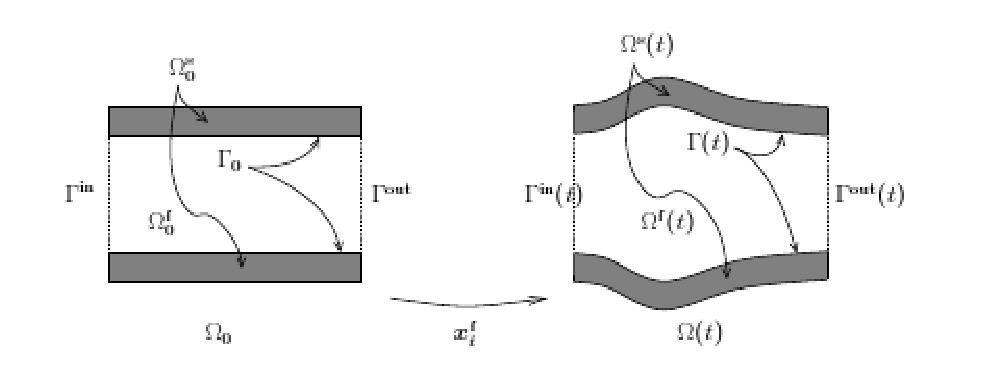
\includegraphics[width=.8\textwidth]{ALEmapping.pdf}
\end{center}
\caption{ALE mapping between the initial configuration and the
configuration at time $t$.}\label{fig:ALEmapping}
\end{figure}

We assume the fluid to be Newtonian, viscous, homogeneous and
incompressible. Its behavior is described by its velocity and
pressure. The elastic solid under large displacements is
described by its velocity and its stress tensor. The classical
conservation laws of the continuum mechanics govern the evolution
of these unknowns.

We denote by $\GamInt$ and $\GamOut$ the inflow and outflow
sections of the fluid domain, by $\uu n_\mf$ the  fluid domain's
outward normal on $\partial \OmegaFt$ and by $\uu n_\ms$ the one
of the structure on the reference boundary $\partial \hOmegaS$.
The boundary conditions on the fluid inlet and outlet can be
either natural or essential (i.e., of Neumann or Dirichlet type,
respectively), while on the interface we impose that the fluid
and structure velocities match and so do the normal stresses. For
simplicity, we assume zero body forces on both the structure and
the fluid and that the boundary conditions on the remaining part
of the structure boundary are of Dirichlet or of Neumann type.

The problem consists in finding the time evolution of the
configuration $\OmegaFt$, as well as the velocity $\uu u$ and
pressure $p$ for the fluid and the displacement $\D$ of
the structure. We define the ALE mapping
\begin{equation*}
 \forall t \,,\;  \ALE{t} : \hOmegaF \rightarrow \OmegaFt,
\end{equation*}
i.e. a map that retrieves at each time the current configuration
of the computational domain $\OmegaFt$. Note in particular that on
the reference interface $\hWall$, $\uu n_\mf \circ \ALE{t} = -\uu
n_\ms$. We denote by $\bY$ the coordinates on the reference
configuration $\hOmegaF$ and by $\bw=\frac{d \ALE{t}}{dt}$ the
domain velocity.

%%%%%%%%%%%%%%%%%%%%%%%%%%%%%%%%%%%%%%%%%%%%%%%%%%%%%%%%%%%%%%%%%%%%%%
\medskip
For simplicity, we denote in short by $\NS(\ldots)$ and
$\Str(\ldots)$ the fluid and structure problems, respectively.
Precisely, for given vector functions $\uu u_\In$, $\uu g_\mf$ and
$\uu f_\mf$, $\NS(\U,p,\ALE{t};\uu u_\In, \uu g_\mf, \uu f_\mf)$
means that we consider the following problem whose solution is
$\U$, $p$ and $\ALE{t}$:
\begin{equation}\label{eq:fluid}
  \NS(\U,p,\ALE{t};\uu u_\In, \uu g_\mf, \uu f_\mf):
  \begin{cases}
    \dis  \uu \Delta \ALE{t} = 0 \text{ in } \hOmegaF, \\
    \dis  \ALE{t} = 0 \text{ on } \partial\hOmegaF \setminus\hat\Sigma, \\
    \dis  \OmegaF_{t} = \ALE{t}(\hOmegaF), \\
    \dis  \rho_\mf\left(\diffALE \U + (\U-\bw)\cdot \Grad \U\right) \\
    \dis  \qquad = \Div (2\mu\uu \epsilon(\U)) - \Grad p  + \uu f_\mf \text{ in }\OmegaF_{t}, \\
    \dis  \Div\U=0 \text{ in }\OmegaF_{t},\\
    \dis  \U = \uu u_\In \text{ on } \GamIn_t,\\
    \dis  \uu\sigma_\mf (\uu u,p)\cdot\uu n_\mf = \uu g_\mf \text{ on }\GamOu_{t},
  \end{cases}
\end{equation}
where $\rho_\mf$ is the fluid density, $\mu$ its viscosity,
$\strain(\U) = \Strain u$ is the strain rate tensor and $\uu
\sigma_\mf(\U,p)=-p Id + 2\mu\strain(\U)$ the Cauchy stress
tensor ($ Id $ is the identity matrix). Note
that~(\ref{eq:fluid}) does not univocally define a solution
$(\U,p,\ALE{t})$ as no boundary data are prescribed on the
interface $\Sigma_t$.

Similarly, for given vector functions $\uu g_\ms$, $\uu f_\ms$, $\Str(\D;\uu g_\ms, \uu f_\ms)$ means that
we consider the following problem whose solution is $\D$:
\begin{equation}\label{eq:struct}
  \Str(\D;\uu g_\ms, \uu f_\ms) :
  \begin{cases}
    \dis  \rho_\ms \frac{\partial^2 \D}{\partial t^2} = \Div(\uu \sigma_\ms(\D))
    -\gamma \D +\uu f_\ms \text{ in }\hOmegaS, \\
    \dis  \uu\sigma_\ms(\D) \cdot {\uu n}_\ms = \uu g_\ms
    \text{ on }\partial\hOmegaS\setminus\hGamW,
  \end{cases}
\end{equation}
where $\piola(\D)$ is the first Piola--Kirchoff stress tensor,
$\gamma$ is a coefficient accounting for possible viscoelastic
effects, while $\uu g_\ms$ represents the normal traction on
external boundaries. Appropriate models have to be chosen for the
structure depending on the specific problem at hand.

Similarly to what we have noticed for~(\ref{eq:fluid}),
problem~(\ref{eq:struct}) can not define univocally the unknown
$\D$ because a boundary value on $\hGamW$ is missing.

When coupling the two problems together, the ``missing'' boundary
conditions are indeed supplemented by suitable matching
conditions on the reference interface $\hWall$. More precisely,
if we denote by $\lambda$ the interface variable corresponding to
the displacement $\D$ on $\hWall$, at any time the coupling
conditions on the reference interface $\hWall$ are
\begin{equation}\label{eq:condizioni}
\begin{array}{c}
  \ALE{t} = \lambda ,\\[4pt]
  \U \circ \ALE{t} = \dot{\D}_{\hWall} ,\\[4pt]
  (\uu \sigma_\mf(\U,p) \cdot {\uu n}_\mf) \circ \ALE{t} +
  \uu \sigma_\ms(\D)\cdot {\uu n}_\ms =0,
\end{array}
\end{equation}
where $\dot{\D}_{\hWall}$ denotes the temporal derivative of
$\D_{\vert\hWall}$. The system of equations (\ref{eq:fluid})-(\ref{eq:condizioni})
identifies our coupled fluid-structure problem.
We suppose the problem to be discretized in time. When the
solution is available at time $t^n$, we look for the solution at
the new time level $t^{n+1} = t^n + \delta t$. If no ambiguity
occurs,  all the quantities will be referred to at time
$t=t^{n+1}$.
Without loss of generality we consider zero body forces, i.e.,
$\uu f_\mf =0$ and $\uu f_\ms=0$.

If we are given a displacement of the interface  $\lambda(t^{n+1})$ at the
time $t^{n+1}$, we can find its harmonic extension on the fluid domain by solving
the  following variational formulation of
(\ref{eq:harmonicextension}):

find $\Df_{t^{n+1}} \in H^1(\DomFi)^3$ such that
\begin{equation} \label{eq:variationalvelocity2}
\left\{
\begin{array}{rcl}
\dis \int_{\DomFi} \Grad \Df_{t^{n+1}}\cdot \Grad \uu \phi  =  0 & & \forall \uu \phi \in H^1_0(\DomFi)^3\\
\Df_{t^{n+1}} = \lambda({t^{n+1}}) & & \text{on } \GamFSi,
\end{array}
\right.
\end{equation}
completed with appropriate boundary conditions  on $\GamIn\cup\GamOu$.

Then we compute the velocity of the fluid domain as 
$\dis \wf{}^{,n+1}_{|\GamFS{n+1}} = 1/\delta t\,(\Df_{t^{n+1}}{}_{|\GamFSi} - \Df_{t^n}{}_{|\GamFSi})
\circ(\ALE {t^{n+1}})^{-1}$ and the velocity and pressure of the fluid at time
$t^{n+1}$ by solving:

find $(\U^{n+1},p^{n+1}) = (\U(t^{n+1}),p(t^{n+1})) \in V^\mf(t^{n+1})\times Q^\mf(t^{n+1})$ such
that $\U^{n+1}_{|\GamFS{n+1}} =  \wf{}^{,n+1}_{|\GamFS{n+1}}$,
$\U^{n+1}_{|\GamIn(t^{n+1})} =  \U_\In(t^{n+1})$
and
\begin{equation} \label{eq:variationalfluid}
\left\{
\begin{array}{l}
\displaystyle \frac{1}{\delta t}\int_{\DomF(t^{n+1})} \rho_\mf \U^{n+1}\V^\mf
+ \displaystyle \int_{\DomF(t^{n+1})}\rho_\mf [(\U^{n+1} -  \wf{}^{,n+1})\cdot \Grad \U^{n+1}]\V^\mf\\ \quad
\displaystyle + \mu\int_{\DomF(t^{n+1})} \Fstress[{n+1}] \cdot \Grad \V^{\mf}
= \displaystyle \frac{1}{\delta t} \int_{\DomF(t^{n+1})} \rho_\mf \U^n \V^\mf +
\int_{\Gamma^{\mathrm{out}}(t^{n+1})} \uu g_{\mf} \V^\mf \\
\displaystyle \int_{\DomF(t^{n+1})} q^\mf \Div \U^{n+1}  = 0
\end{array}
\right.
\end{equation}
for all $(\V^\mf,q^\mf) \in V_0^\mf(t^{n+1}) \times Q^\mf(t^{n+1})$, with
\begin{eqnarray*}
V^\mf(t) & = & \left\{\V^\mf \vert \,   \V^\mf \circ \ALE {t}  \in H^1(\DomFi)^3\right\}, \\
V_0^\mf(t) & = & \left\{\V^\mf \in V^\mf(t) \vert \,\V^\mf  \circ \ALE {t}
= \mathbf{0} \mbox { on } \GamFSi \cup \GamIn \right\}, \\
Q^\mf (t)& = & \left\{q^\mf  \vert \, q^\mf \circ \ALE {t} \in L^2(\DomFi)\right\},
\end{eqnarray*}
and where the fluid domain $\DomF(t^{n+1})$ is given by
\begin{equation*}
\DomF(t^{n+1})  = \ALE {t^{n+1}}(\DomFi).
\end{equation*}

We can then compute $  (\Fstress[{n+1}] \cdot {\uu n}_\mf) \circ \ALE t $ on $ \GamFSi$,
which by (\ref{eq:couplingconditions}) has to be equal to the structure normal stresses.
%We call $\Sf$ the operator that given $\lambda$ computes $S_\mf(\lambda)= \sigma_\mf$.


On the structure side, given the same displacement $\lambda(t^{n+1})$, we can use the
following scheme to approximate the arterial deformation and the domain
velocity (see \cite{FerMou04:NewtonFS}):

find $(\ds{}^{,n+1},\ws{}^{,n+1})=(\ds(t^{n+1}),\ws(t^{n+1})) \in V^\ms\times
V^\ms$ such that
\begin{equation} \label{eq:variationalstructure}
\left\{
\begin{array}{rl}
%    \dis  \int_{\DomSi} \rho_\ms \frac{\partial^2 \uu d^\ms}{\partial t^2}v^\ms
    \dis  \frac{2}{\delta t^2} \int_{\DomSi} \rho_\ms \ds{}^{, n+1} \V^\ms
    &\dis-  \frac{2}{\delta t^2} \int_{\DomSi} \rho_\ms (\ds{}^{, n} + \delta t \ws{}^{, n})\V^\ms
    +  \int_{\DomSi} \Sstress(\ds{}^{, n+1})\cdot \Grad \V^\ms    \\
    &\dis = \int_{\partial\DomSi\setminus\GamFSi} \uu g_\ms \cdot \V^\ms\\
    \dis \uu w^{\ms,n+1} &\dis=  \frac{2}{\delta t}(\uu d^{\ms,n+1} - \uu d^{\ms,n}) - \ws{}^{,n}\\
    \dis\uu d^{\ms,n+1} &\dis =  \lambda(t^{n+1}) \quad\text{ on } \GamFSi,
    \end{array}
\right.
\end{equation}
for all $\V^\ms \in V^\ms$ such that $\V^\ms_{|\GamFSi} = 0$,
with $V^\ms = H^1(\DomSi)^3 $. As for the fluid, we can then compute the structure
normal stresses on the interface  as $\Sstress(\Ds{}^{, n+1}) \cdot {\uu n}_\ms$  on $\GamFSi$.

If for a given interface displacement $\lambda(t^{n+1})$ the fluid and structure normal stresses are
at equilibrium,
%  i.e.,
% $(\Fstress \cdot {\uu n}_\mf) \circ \ALE t +
% \Sstress(\Ds) \cdot {\uu n}_\ms = 0$,
%$ \sigma_\mf + \sigma_\ms = 0$,
it means that the fluid-structure problem has
been correctly solved.
In general we impose the equilibrium in weak form, i.e.,
\begin{multline*}
  \int_{\GamFS{n+1}} \Fstress \cdot \uu n_{\mf}\V^\mf + \int_{\GamFSi}
  \Sstress(\Ds) \cdot \uu n_{\ms} \V^s = 0 \\
  \forall (\V^\mf,
  \V^\ms) \in V^\mf(t^{n+1}) \times V^\ms \text{ s.t. } \V^\mf\circ\ALE t =
  \V^\ms \text{ on } \GamFSi.
\end{multline*}
Both integrals can be computed as residuals of
the weak form of the equations.
We consider the coupled problem at a particular time  $t=t^{n+1}$.
In order to write the interface equation associated to the global
fluid-structure problem, we introduce a fluid and structure operator
as follows.

Let $\Sf$ be the Dirichlet-to-Neumann (D-t-N) fluid map such that to any given interface
displacement $\lambda$ it associates the normal stress
$$
\Sf (\lambda) = \sigma_\mf :=  (\Fstress \cdot {\uu n}_\mf) \circ \ALE t \mbox{ on } \GamFSi,
$$
where $(\U, p)$ is the solution of the Navier-Stokes problem (\ref{eq:variationalfluid}). On the
other hand, we denote by $\Ss$ the D-t-N operator associated to the structure in $\GamFSi$ such
that to any given displacement $\lambda$ of the interface $\GamFSi$ it associates the normal stress
exerted by the structure on $\GamFSi$:
$$
\Ss (\lambda) = \sigma_\ms :=  (\Sstress(\Ds) \cdot {\uu n}_\ms) \mbox{ on } \GamFSi,
$$
where $\Ds$ is the solution of (\ref{eq:variationalstructure}).

Concerning the inverse of the solid operator, we can define $S_\ms^{-1}$ as a Neumann-to-Dirichlet
(N-t-D) map that at any given normal stress $\sigma$ on $\GamFSi$ associates the interface
displacement $\lambda(t^{n+1}) = \D^{\ms,n+1}$ by solving a structure problem analogous to
(\ref{eq:variationalstructure}), but with the Neumann boundary condition
\begin{equation*}
\uu \sigma_\ms(\D^s) \cdot\uu n_\ms = \sigma \textrm{ on } \GamFSi
\end{equation*}
and then computing the restriction on $\GamFSi$ of the displacement of
the structure domain.

Moreover, we denote by $S_\ms'$ the tangent operator associated to the structure problem and by
$(S_\ms')^{-1}$ its inverse. The latter is a N-t-D map that to any given normal stress $\sigma$ on
$\GamFSi$ associates the corresponding displacement $\lambda(t^{n+1})$ of the interface by solving
the linearized structure problem with boundary condition $\boldsymbol{\sigma}_\ms (\Ds) \cdot \uu
n_\ms = \sigma$ on $\GamFSi$. Analogously, by $(S_\mf')^{-1}$ we denote the inverse of the tangent
operator $S_\mf'$. This is also a N-t-D map  that for any given normal stress $\sigma$ on $\GamFSi$
computes the corresponding displacement $\lambda(t^{n+1})$ of the interface through the solution of
linearized Navier-Stokes equations with the boundary condition $(\Fstress \cdot {\uu n}_\mf) \circ
\uu x^{\mf} = \sigma$ on $\Gamma_0$.
Using the definitions of the operators $\Sf$ and $\Ss$ and of their inverses, we can express the
coupled fluid-structure problem in terms of the solution $\lambda$ of a nonlinear equation defined
only on $\GamFSi$. More precisely, we can envisage three possible formulations for the interface
equation which are all equivalent from a mathematical point of view, but give rise to different
iterative methods.

First, we have the fixed-point formulation
\begin{equation} \label{eq:fixedpoint}
\mbox{find } \lambda \mbox { such that } \Ss^{-1}(-\Sf(\lambda)) = \lambda
\mbox{ on } \GamFSi .
\end{equation}
This is a classical formulation in fluid-structure interaction problems, but it is worth pointing
out that here the fixed point is the displacement of the sole interface, whereas in the
literature the solution obtained via
fixed-point algorithms usually represents the displacement of the whole solid domain.

The second possible approach is a slight modification of the previous equation
(\ref{eq:fixedpoint})
\begin{equation} \label{eq:newton}
\mbox{find } \lambda \mbox { such that } \Ss^{-1}(-\Sf(\lambda)) - \lambda = 0 \mbox{ on } \GamFSi,
\end{equation}
which is more suitable for setting up a Newton iterative method.
Again, this is applied solely to the interface displacement,
instead of the whole solid displacement as proposed.

Let's have a look at the code located at \verb!testsuite/test_fsi/main.cpp!. The first interesting part
is the problem definition part, starting from these lines 
\begin{verbatim}
    Problem( GetPot const& data_file, std::string _oper = "" )
        {
            using namespace LifeV;

            Debug( 10000 ) << "creating FSISolver with operator :  " << _oper << "\n";

            M_fsi = fsi_solver_ptr(  new FSISolver( data_file, _oper ) );
            Debug( 10000 ) << _oper << " set \n";

            MPI_Barrier(MPI_COMM_WORLD);
\end{verbatim}

This will create a new fluid/structure interaction problem that will be solved using a
non-linear Richardson algorithm on the following interface equation 

\begin{equation}\label{eqn-interface}
\lambda^{k+1}  =  \lambda^k + \omega^k f(\lambda^k),
\end{equation}
where $f$ depends on the chosen FSI method. If we look at the FSI problem constructor
the file \verb!life/lifesolver/FSISolver.cpp!, we have 

\begin{verbatim}
FSISolver::FSISolver( GetPot const& data_file,
                      std::string   __oper ):
    M_lambda      (),
    M_lambdaDot      (),
    M_firstIter (true),
    M_method    ( data_file("problem/method"     , "steklovPoincare") ),
    M_maxpf     ( data_file("problem/maxSubIter" , 300) ),
    M_defomega  ( data_file("problem/defOmega"   , 0.01) ),
    M_abstol    ( data_file("problem/abstol"     , 1.e-07) ),
    M_reltol    ( data_file("problem/reltol"     , 1.e-04) ),
    M_etamax    ( data_file("problem/etamax"     , 1.e-03) ),
    M_linesearch( data_file("problem/linesearch" , 0) ),
    M_epetraComm(),
    M_epetraWorldComm(),
    M_localComm (new MPI_Comm),
    M_interComm (new MPI_Comm),
    out_iter    ("iter"),
    out_res     ("res")
\end{verbatim}


where
\begin{itemize}
\item \verb!M_lambda! is the interface displacement as defined in (\ref{eq:condizioni}),
\item \verb!M_lambdaDot! is the temporal derivative of \verb!M_lambda!.
\end{itemize}
See table \ref{table-fsiparams} for a complete of these options of options.

\begin{table}[!h]
\begin{center}
\begin{tabular}{|l|l|l|}
\hline
Name & Options & Description \\
\hline \hline
method & fixedPoint & FSI resolution method name\\
& exactJacobian & \\
\hline
maxSubIter & 300 & maximum nonlinear Richardson iterations \\
\hline
defOmega & 0.01 & default step in (\ref{eqn-interface}) (deprecated) \\
\hline
abstol & 1e-07 & abstol and reltol define the stoping \\
reltol & 1e-04 & criteria as abstol+reltol*norm(residual0) \\
& & where residual0 is the first nonlinear Richardson \\
& & FSI evaluation residual. \\
\hline
etamax & 1e-03 &  Maximum error tolerance for residual in the linear solver. \\
\hline
linesearch & 0 & nonlinear Richardson algorithm linesearch \\
& & (always use 0, i.e no line search, for now).\\
monolithic & 0 & monolithic description of the FSI problem \\
& & (under development)\\
\hline

\end{tabular}
\end{center}
\caption{ FSI problem data file parameters
%\ixt{FSI data parameters}{data parameters}
}
\label{table-fsiparams}
\end{table}


The \verb!monolithic! description of the FSI problem is still under  development and
should not be used for now. Let's have the look at the rest of the FSI problem constructor code.

\begin{verbatim}
 MPI_Group  originGroup, newGroup;
 MPI_Comm   newComm;

 MPI_Comm_group(MPI_COMM_WORLD, &originGroup);

 if (numtasks == 1)
     {
         std::cout << "Serial Fluid/Structure computation" << std::endl;
         newComm = MPI_COMM_WORLD;
         fluid = true;
         solid = true;
         fluidLeader = 0;
         solidLeader = 0;

         M_epetraWorldComm.reset(new Epetra_MpiComm(MPI_COMM_WORLD));
         M_epetraComm = M_epetraWorldComm;

     }
 else
     {
         int members[numtasks];

         solidLeader = 0;
         fluidLeader = 1 - solidLeader;

         if (rank == solidLeader)
             {
                 members[0] = solidLeader;
                 int ierr;
                 ierr = MPI_Group_incl(originGroup, 1, members, &newGroup);
                 solid = true;
             }
         else
             {
                 for (int ii = 0; ii <= numtasks; ++ii)
                     {
                         if ( ii < solidLeader)
                             members[ii] = ii;
                         else if ( ii > solidLeader)
                             members[ii - 1] = ii;
                     }
                 int ierr;
                 ierr = MPI_Group_incl(originGroup,
                                       numtasks - 1,
                                       members,
                                       &newGroup);
                 fluid = true;
             }

         MPI_Comm* localComm = new MPI_Comm;
         MPI_Comm_create(MPI_COMM_WORLD, newGroup, localComm);
         M_localComm.reset(localComm);

         M_epetraComm.reset(new Epetra_MpiComm(*M_localComm.get()));
         M_epetraWorldComm.reset(new Epetra_MpiComm(MPI_COMM_WORLD));
     }

\end{verbatim}

This part is dedicated at assigning jobs to the different processors. Since we have to deal
with a separate structure and fluid problems, we define two MPI groups where for each problem.
For now, by convention, and since the structure problem is resolved more easily than the
fluid problem by far, the structure group has only the \#0 (leader) processor, whereas the fluid group is
composed of all the other processors. At the end of these lines, two MPI intracommunicators
(communicator within a single group of processes), one for the structure,
one for the fuid, and one MPI intercommunicator (communicator within two or
more groups of processes) are created. See \url{http://www.mpi-forum.org/docs/mpi-11-html/mpi-report.html}
for more information on intra and intercommunicators.

From now on, each processor knows if it belongs to the structure or the fluid group. This is
very important since each group will create its own problem, either stucture of fluid.
Since the structure problem requires less ressources than the fluid problem, the FSI problem defined in (\ref{eqn-interface})
will be solved on a lead structure processor (\#0 processor within the structure intracommunicator).

\begin{verbatim}


    Preconditioner precond  = ( Preconditioner )
                               data_file("problem/precond"   ,
                               DIRICHLET_NEUMANN );

    Debug( 6220 ) << "FSISolver::preconditioner: " << precond << "\n";

    if ( !__oper.empty() )
    {
        M_method = __oper;
    }

    Debug( 6220 ) << "FSISolver::setFSIOperator " << M_method << "\n";

    this->setFSIOperator( M_method );

    M_oper->setFluid(fluid);
    M_oper->setSolid(solid);

    M_oper->setFluidLeader(fluidLeader);
    M_oper->setSolidLeader(solidLeader);

    Debug( 6220 ) << "FSISolver::setPreconditioner " << precond << "\n";

    std::cout << std::flush;
    M_oper->setComm(M_epetraComm, M_epetraWorldComm);

    Debug( 6220 ) << "FSISolver::setDataFromGetPot " << precond << "\n";
    std::cout << std::flush;

    M_oper->setDataFromGetPot( data_file );


    Debug( 6220 ) << "FSISolver::setPrecond " << precond << "\n";
    std::cout << std::flush;

    M_oper->setPreconditioner( precond );

    M_oper->setup();

    Debug( 6220 ) << "FSISolver:: variable setup " << precond << "\n";

    M_oper->setUpSystem(data_file);

    M_lambda.reset   (new vector_type(*M_oper->solidInterfaceMap()));
    M_lambdaDot.reset(new vector_type(*M_oper->solidInterfaceMap()));
    M_oper->buildSystem();

\end{verbatim}

This part  creates the proper numerical FSI Operator (fixed point, exact jacobian, ...)
for solving (\ref{eqn-interface}), that is the fluid and the structure operators ($S_f$, $S_s$ ... )
defined previously, and set them up. You can have a look at the code which is in \verb!life/lifesolver/FSIOpertator.hpp,cpp!,
\verb!life/lifesolver/exactJacobianBase.hpp,cpp! and \verb!life/lifesolver/fixedPointBase.hpp,cpp!.
The last two classes, exactJacobian and fixedPoint, derive from the class FSIOperator, which only
deals with passing information (displacement or constrain) from the solid or the fluid to the fluid or solid via
the interface. The the specialized classes exactJacobian or fixedPoint evalute the interface residual
and solve $f(\lambda)$ as defined in (\ref{eqn-interface}).
The last interesting part in the \verb!FSISolver! class, is the \verb!iterate! member
\begin{verbatim}
    M_oper->setTime(time);

    fct_type fluidSource(zero_scalar);
    fct_type solidSource(zero_scalar);

    if(!M_monolithic)
        M_oper->updateSystem(fluidSource, solidSource);
    else
        M_oper->updateSystem(*M_lambda);

    // displacement prediction
    MPI_Barrier(MPI_COMM_WORLD);

    if (M_firstIter)
    {
        M_firstIter = false;

        if(!M_monolithic)
            {
                *M_lambda      = M_oper->lambdaSolid();
                *M_lambda     += timeStep()*M_oper->lambdaDotSolid();
                *M_lambdaDot   = M_oper->lambdaDotSolid();
            }
    }
    else
    {

        if(!M_monolithic)
            {
                *M_lambda      = M_oper->lambdaSolid();
                *M_lambda     += 1.5*timeStep()*M_oper->lambdaDotSolid(); // *1.5
                *M_lambda     -= timeStep()*0.5*(*M_lambdaDot);
                *M_lambdaDot   = M_oper->lambdaDotSolid();
            }
    }


    if (!M_monolithic)
        {
            M_oper->leaderPrint("norm( disp  ) init = ", M_lambda->NormInf() );
            M_oper->leaderPrint("norm( velo )  init = ", M_lambdaDot->NormInf());
        } else {
            M_oper->leaderPrint("norm( solution ) init = ", M_lambda->NormInf() );
        }

    MPI_Barrier(MPI_COMM_WORLD);

    int maxiter = M_maxpf;

    // the newton solver
    UInt status = 1;
    Debug( 6220 ) << "Calling non-linear Richardson \n";

    status = nonLinRichardson(*M_lambda,
                              *M_oper,
                              norm_inf_adaptor(),
                              M_abstol,
                              M_reltol,
                              maxiter,
                              M_etamax,
                              M_linesearch,
                              out_res,
                              time);

    if(status == 1)
    {
        std::ostringstream __ex;
        __ex << "FSISolver::iterate ( " << time << " )
                 Inners iterations failed to converge\n";
        throw std::logic_error( __ex.str() );
    }
    else
    {
        M_oper->leaderPrint("End of time " , time);
        M_oper->leaderPrint("Number of inner iterations       : ", maxiter );
        out_iter << time << " " << maxiter << " "
                 << M_oper->nbEval() << std::endl;
    }
    if(!M_monolithic)
        M_oper->shiftSolution();

\end{verbatim}

This code will perform one FSI time step. First, it ``guesses'' the interface
displacement by interpolation of the previous displacement, then it will call the
non-linear Richardson algorithm that will compute the new displacement by solving
(\ref{eqn-interface}).







%
%%%%%%%%%%%%% Some Settings for emacs and auc-TeX
% Local Variables:
% TeX-master: t
% TeX-command-default: "PDFLaTeX"
% TeX-parse-self: t
% TeX-auto-save: t
% x-symbol-8bits: nil
% TeX-auto-regexp-list: TeX-auto-full-regexp-list
% eval: (ispell-change-dictionary "american")
% End:
%


\bibliographystyle{plain}
\bibliography{lifev}

\printindex

\end{document}
